We chose computational group theory (CGT) to conduct a case study in creating MitM ontologies. CGT is one of the oldest computational mathematics disciplines and the knowledge covered in \GAP and its organization already provides a strong template for the MitM ontology. The formalization can be found at~\cite{mitm:groups:on}.

\subsection{The Foundation for MitM}
As foundation for all formalizations in MitM~\cite{mitm:foundation:on} we use a polymorphic extension of LF, a dependently typed $\lambda$-calculus using a hierarchy
of two universes \lstinline|type| and \lstinline|kind|, where \lstinline|type:kind| (roughly analogous to sets and proper classes in set theory). 
LF merely provides dependent function types \lstinline|{a:A}B(a)|, representing the type of all functions mapping an argument \lstinline|a:A| to some element of type \lstinline|B(a)|; if \lstinline|B| does not depend on the argument \lstinline|a|, we obtain the simple function type \lstinline[mathescape]|A$\to$B|. 

For axioms and theorems (being expressions of a primitively declared type \lstinline|prop|), we use on top of that a higher order logic where quantifiers range over any type. We furthermore follow the judgments-as-type paradigm by declaring a function \lstinline[mathescape]|$\vdash$:prop$\to$type| mapping propositions to the \emph{type of their proofs}, which allows us to declare proof rules as functions mapping proofs (of the premises) to a proof (of the conclusio).

We furthermore add various subtyping principles; among them declared subtypes (where constants of LF-type \lstinline|A<:B| are seen as declaring that \lstinline|A| is a subtype of \lstinline|B|), power types (being the type of all subtypes of some given type) and predicate subtyping \lstinline?{'a:A | P(a)'}? (representing the type of all \lstinline|a:A| for which the type \lstinline|P(a)| is inhabited). The latter necessarily introduces undecidability, but for our purposes this is unproblematic. These features turned out to be necessary to formalize many areas of mathematics close to their usual informal treatment, as e.g. when talking about properties of special subgroups, topological subspaces and similar situations.

\begin{wrapfigure}r{6.1cm}\vspace*{-2.5em}
  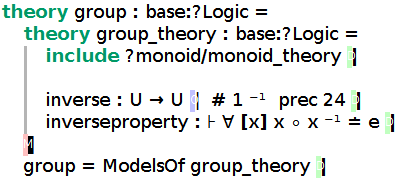
\includegraphics[width=.5\textwidth]{mitm1}\vspace*{-1em}
  \caption{MitM ontology Fragment}\label{fig:mitm1}\vspace*{-1em}
\end{wrapfigure}
 Additionally we extend our type theory with \emph{record types} as well as a convenience operator \lstinline|ModelsOf|, taking a \emph{theory} as argument and returning a record type. The (typed, but) undefined constants of the theory are turned into fields of the resulting record type, which allows us to think of the record type \lstinline|ModelsOf T| as the type of models of the theory \lstinline|T|. This enables us to e.g. define a group by simply giving the theory of its signature and (first-order) axioms, while still giving us a type \lstinline|group=ModelsOf group_theory| of all groups, as seen in Figure~\ref{fig:mitm1}. Any element \lstinline|g:group| thus represents an actual group, whose operations and axioms can be accessed via record field projections (e.g. \lstinline|g.inverse| yields the inverse operation of \lstinline|g|, which has type \lstinline[mathescape]|g.U$\to$g.U|). Since axioms are turned into record type fields as well, to actually construct a record of type \lstinline|group| corresponds to proving that the field \lstinline|universe| and the operations provided in the record do in fact form a group.


\subsection{Layers of Abstraction}

Our formalisation of CGT follows the template of its implementation in \GAP, and requires
different levels of abstraction, currently \emph{abstract}, \emph{representation},
\emph{implementation}, and \emph{concrete}.  From our experience, we expect this pattern
to be applicable across computational algebra, possibly with additional levels of
abstraction. The left box in Figure \ref{fig:cgtontology} shows the levels and which level
various constructors and operations of the \GAP system dialect belong to.

\begin{figure}[ht]\centering
  \tikzinput[width=.98\textwidth]{alignmentimg}
  \caption{Alignments between the MitM Ontology and the \GAP API}\label{fig:cgtontology}
\end{figure}
\ednote{MK@MP: there must be other symbols at the lower levels; can you give them?}

\paragraph{Abstract Level} This contains the theory of \emph{Groups}: the group axioms, generating sets, homomorphisms, group actions, stabilisers, and orbits.  
This also easily leads into definitions of centralisers -- i.e. stabilisers of elements under conjugation -- and normalisers -- i.e. stabilisers of subgroups under conjugation, stabiliser chains, Sylow-$p$ subgroups, Hall subroups, and many other concepts.

\OMMT also allows expressing that there are different equivalent definitions of a concept: We defined group actions in two ways and used \emph{views} to express their equivalence.

\paragraph{Representation Level} 
Abstract groups can be represented in many ways as concrete mathematical
objects suitable for computation: as groups of permutations, groups of matrices,
finitely presented groups, or using a polycyclic presentation.

Additionally, mathematicians often compute with canonical representatives of an isomorphism class of groups: When group theorists talk about the ``Dihedral group of order 8'', they often have a particular representation in mind, for example as a group that acts on the square by rotations and reflections. 
In \GAP this group would be represented as a group of permutations, or by a polycyclic presentation.

Many representations arise naturally from \emph{group actions}: If we are
considering symmetry in a setting where we want to apply group theory, we start
with a group action.\ednote{MP@ALL: More concrete? More ``gripping''? I already
talked about the canonical example with the dihedral group}

The universal tool to bridge the gap between groups, representations and
canonical representatives are group homomorphisms, particularly isomorphisms,
which are used extensively in \GAP. This is reflected in our approach.

\paragraph{Implementation Level}
At the lowest level there are implementation details: Permutation groups in \GAP
are considered as finite subgroups of the group $S_{\mathbb{N}+}$, and defined by
providing a set of generating permutations. \GAP then computes a stabiliser chain
for a group that was defined this way, and naturally considers the group to be a
subgroup of $S_{[1..n]}$, where $n$ is the largest point moved.

\paragraph{Concrete Level}\ednote{MK: where is the promised concrete level?}

\paragraph{Evaluation}
Building this part of the CGT MitM Ontology already posed a few challenges for
the \MMT system, mostly to do with subtyping, since we needed to be able to talk
about all subgroups of a group, and all normal subgroups of a group. Quantifying
over these classes can lead to inconsistencies in the underlying type theory.
These challenges immediately translate into necessary
features in \OMMT, for example by introducing universe hierarchies.
\ednote{MP@FR+DM: Is this too gratuitous? Not concrete enough?}

%%% Local Variables:
%%% mode: latex
%%% TeX-master: "paper"
%%% End:

%  LocalWords:  sec:cgt MueRoYuRa:abtafs17,MueGauKal:cacfms17 emph Sylow subroups medskip formalizations mcpoot13 wrapfigure vspace
%  LocalWords:  mathbb fig:cgtontology alignmentimg smallskip subtyping organization
%  LocalWords:  centering tikzinput textwidth rotercentations lstinline lstinline vdash
%  LocalWords:  type:kind mathescape conclusio fig:mitm1 g:group includegraphics mitm1
